\documentclass[11pt,a4paper]{article}
\usepackage{ngerman}
\usepackage[ngerman]{babel}
\usepackage[utf8x]{inputenc}
\usepackage[T1]{fontenc}
\usepackage{lmodern}
\usepackage{marvosym}
\usepackage{amsfonts,amsmath,amssymb}
\usepackage{textcomp}
\usepackage{pifont}
\usepackage{ifpdf}
\usepackage[pdftex]{color}
\ifpdf
  \usepackage[pdftex]{graphicx}
\else
  \usepackage[dvips]{graphicx}\fi

\pagestyle{empty}

\usepackage[scale=0.775]{geometry}
\setlength{\parindent}{0pt}
\addtolength{\parskip}{6pt}

\def\firstname{Pascal}
\def\familyname{Bernhard}
\def\FileAuthor{\firstname~\familyname}
\def\FileTitle{\firstname~\familyname's Reformation}
\def\FileSubject{Reformation}
\def\FileKeyWords{\firstname~\familyname, Reformation}

\renewcommand{\ttdefault}{pcr}
\hyphenation{ins-be-son-de-re}
\usepackage{url}
\urlstyle{tt}
\ifpdf
  \usepackage[pdftex,pdfborder=0,breaklinks,baseurl=http://,pdfpagemode=None,pdfstartview=XYZ,pdfstartpage=1]{hyperref}
  \hypersetup{
    pdfauthor   = \FileAuthor,%
    pdftitle    = \FileTitle,%
    pdfsubject  = \FileSubject,%
    pdfkeywords = \FileKeyWords,%
    pdfcreator  = \LaTeX,%
    pdfproducer = \LaTeX}
\else
  \usepackage[dvips]{hyperref}
\fi

\definecolor{firstnamecolor}{RGB}{56,115,179}
\definecolor{familynamecolor}{RGB}{56,115,179}
\hypersetup{pdfborder=0 0 0}

% Gleiche Schriftart für Hyperlinks
\urlstyle{same}


%  Gefrickel um URL-Links vernünftig umzubrechen
\makeatletter
\g@addto@macro\UrlBreaks{
  \do\a\do\b\do\c\do\d\do\e\do\f\do\g\do\h\do\i\do\j
  \do\k\do\l\do\m\do\n\do\o\do\p\do\q\do\r\do\s\do\t
  \do\u\do\v\do\w\do\x\do\y\do\z\do\&\do\1\do\2\do\3
  \do\4\do\5\do\6\do\7\do\8\do\9\do\0}
% \def\do@url@hyp{\do\-}

% Hiermit soll einer übervolle Box verhindert werden -- funktioniert sogar irgendwie
\g@addto@macro\UrlSpecials{\do\/{\mbox{\UrlFont/}\hskip 0pt plus 1pt}}
\makeatother

% Farben werden hier definiert
\definecolor{MidnightBlue}{RGB}{0,103,149}


\begin{document}
\sffamily   % for use with a résumé using sans serif fonts;
%\rmfamily  % for use with a résumé using serif fonts;
\hfill%
\begin{minipage}[t]{.6\textwidth}
\raggedleft%
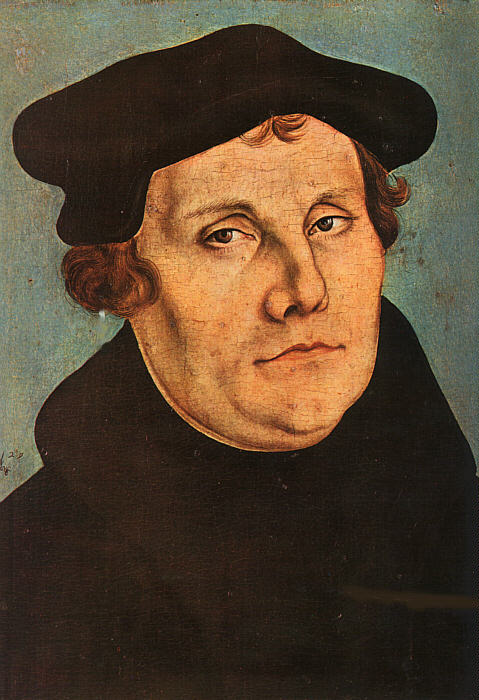
\includegraphics[width=0.55\textwidth]{Martin_Luther.jpg}


%	{\bfseries {\color{firstnamecolor}\firstname}~{\color{familynamecolor}\familyname}}\\[.35ex]
%	\small\itshape%
%	Schwalbacher Straße 7\\
%	12161 Berlin\\[.35ex]
%	\Mobilefone~+49 162 32 39 557 \\
%	\Letter~\href{mailto:pascal.bernhard@rppr.de}{pascal.bernhard@rppr.de}
\end{minipage}\\[0.5em]
%
{\color{firstnamecolor}\rule{\textwidth}{.25ex}}
%
\begin{minipage}[t]{.4\textwidth}
	\raggedright%
	% {\bfseries {\color{firstnamecolor}
	\vspace*{1em}
	\textbf{Reformation -- Gegenreformation -- Glaubenskriege} \\
%	 \\[.35ex]
	% }}
	\small%
%	Wolframstraße 89-92\\
%	12105 Berlin
\end{minipage}
%
\hfill
%
\begin{minipage}[t]{.4\textwidth}
	\raggedleft % US style
	\today
	%April 6, 2006 % US informal style
	%05/04/2006 % UK formal style
\end{minipage}\\[2.2em]


{\bfseries \color{familynamecolor}{Die Reformation und Glaubensspaltung in Europa}}\\[0.75em]

\section*{\textsf{Auslöser und Faktoren der Reformation}}

\begin{itemize}
\item Spaltung der westlichen Christenheit - Erneuerungsbewegung (1517-1648)
\item Beginn der Reformation wird auf Luthers Anschlag seiner 95 Thesen an die Wittenberger Schlosskirche datiert
\item die Reformation wurde angeführt von Martin Luther (Deutschland), sowie Huldrych Zwingli und Johannes Calvin (Schweiz)
\item anfänglich war die Reformationsbewegung der Versuch, die katholische Kirche zu reformieren, es sollte keine neue Kirche gegründet oder ein Schisma herbeigeführt werden


\item Renaissance und humanistisches Denken führen zu einer kritischen Auseinandersetzung mit Gegenwart und ihren Verhältnissen
\item ein zunehmender Anteil der Bevölkerung konnte lesen und schreiben (Händler, aufkommenden Bürgertum in den Städten)
\item der Buchdruck und Einsatz beweglicher Lettern machte es möglich Information schnell und über große Distanzen zu verbreiten\\
	\ding{225} das Buch wurde zum Massenmedium\\


\end{itemize}


\subsection*{\textsf{Religiöse Faktoren}}

\begin{itemize}
\item Kritikpunkte an der katholischen Kirche (falsche Lehren und Missbrauch):

	\begin{enumerate}
	\item Ablassbriefe
	\item \textsl{Simonie} (Ämterkauf)
	\item \textsl{Nepotismus} (Vergabe von Ämtern an Verwandte)
	\item allgemeine Korruption in der Kirche (katholische Kirche beanspruchte absolute moralische Authorität und Vorbildfunktion, die sie nicht erfüllte)
	\end{enumerate}

\item starke Frömmigkeit nach Todeserfahrungen mit der Pest

	\begin{itemize}
	\item Wunsch, seine Sünden reinzuwaschen, um so unsündig vor das jüngste Gericht treten zu können
	\item Kirche nutzte dieses Verlangen nach Vergebung der Sünden durch System der Ablassbriefe aus\\
	\ding{225} Religion wurde sozusagen 'fiskalisiert'
	\item der damalige Papst Julius II brauchte dringend Geld für den Neubau des Petersdoms, daher wurde der Ablasshandel forciert
	\end{itemize}


\item Papst handelte wie ein weltlicher Fürst (führte Kriege, lebte im Luxus)

\item gegenseitige Exkommunikation der Päpste während des abendländischen Schismas (1378-1417)\\
\ding{225} die Bedeutung des Paptstums war in den Augen vieler Gläubiger relativiert worden

\item \textbf{Anspruch und Wirklichkeit der Heilsanstalt \textsl{Kirche} klafften zunehmend auseinander}\\
\ding{225} die Kirche verlor an Glaubwürdigkeit auch in religiösen Fragen



\end{itemize}


\subsection*{\textsf{Politische Situation in Europa}}

\begin{itemize}
\item \textbf{Gegensatz zwischen Habsburg und Frankreich:}
	
	\begin{itemize}
	\item Karl V. von Spanien und Fran\c{c}ois Ier führten zwischen 1521 und 1544 drei Kriege in Italien um die dortige Vormachtstellung
	\item Frankreich waren zwischen habsburgischen Territorien eingeklammert (Spanien im Süden; habsburgische Niederlande im Norden; Österreich im Osten)
	\end{itemize}
\item Gefahr der Türken im Osten (Belagerung Wiens 1529)\\
\ding{225} Deutscher Kaiser, zugleich König Österreich brauchte Geld und Truppen gegen die Türken\\
\ding{225} Unterstützung der Reichsstände im Reichstag, wodurch seine Position gegenüber den Reichsfürsten geschwächt wurde



\end{itemize}


\section*{\textsf{Weshalb nahm die Reformation in Deutschland ihren Ausgang?}}


\begin{itemize}
\item die wirtschaftliche Situation des Großteils der Bevölkerung verschlechterte sich im 16. Jahrhundert
\item die meisten Menschen lebten am Existenzminimum
\item starkes Bevölkerungswachstum (von 12 auf 15 Million in Deutschland) zwischen 1500 und 1600
\item Arbeitskraft verbilligte sich (sinkende Löhne) bei steigenden Lebensmittelpreisen
\item durch den großen Zustrom an Gold aus Lateinamerika sank der Geldwert\\
\ding{255} Inflation traf Leute, die von Lohneinkommen lebten am stärksten (Armensteuer)

\vspace{1cm}

\item es gab im Heiligen Deutschen Reich keine Zentralinstanz, die Glaubensfragen allgemeingültig hätte klären können
\item Vielzahl an relative autonomer Territorien führte zu einer konfessionellen Fragmentierung
\item der deutsche Kaiser konnte die Spaltung nicht verhindern, da ihm die Macht hierzu fehlt, obwohl er dies wollte
\end{itemize}

\section*{\textsf{Gedanken der Reformation}}

\begin{itemize}
\item Martin Luther wendete sich Gerechtigkeitsverständnis der \textsl{iustitia distributiva} ab (Jeder bekommt das, was ihm zusteht) und der Konzeption der \textsl{iustitia passive} zu (Gott ist gerecht, indem er gerecht macht, allen steht Gerechtigkeit zu)\\
\ding{225} \textsl{Der Sünder kann seine Rechtfertigung und Gerechtigkeit nicht durch Werke, wie der Kauf von Ablassbriefen verdienen, sondern erfährt sie durch den Glauben an Gott}
\item Es kommt auf die innere Reue der Gläubigen an, nicht die Kirche kann dies vermitteln
\item Luther propagierte in späteren Schriften die Abschaffung des Zölibats sowie des Kirchenstaates
\item das hierarchische System zwischen Klerus und Laien wurde kritisiert
\item Rückbesinnung auf die Bibel, die Heilige Schrift hat Vorrang vor den Lehren der Kirche

\item \textbf{Grundlagen der reformatorischen Theologie:}

	\begin{itemize}
	\item Allein durch die Gnade Gottes wird der glaubende Mensch errettet, nicht durch seine Werke.
	\item Allein durch den Glauben wird der Mensch gerechtfertigt, nicht durch gute Werke.
	\item Allein die Schrift ist die Grundlage des christlichen Glaubens, nicht die kirchliche Tradition.
	\item Allein die Person, das Wirken und die Lehre Jesu Christi können Grundlage für den Glauben und die Errettung des Menschen sein.
	\end{itemize}

\item Martin Luther übersetzte das Neue Testament neu und verwendete hierfür eine volkstümliche, verständliche Sprache
\item die Bibel wurde nun für größere Teile der deutschen Bevölkerung verständlich
\item Laien waren nicht mehr auf die Interpretation der katholischen Priester angewiesen\\
\ding{225} die katholische Kirche verlor die Deutungshoheit über die Heilige Schrift
\item Wissen ist Macht\\
\ding{225} \textbf{Das theologische Machtmonopol der katholischen Kirche war gebrochen}



\end{itemize}


\end{document}